\documentclass[tikz,border=2pt]{standalone}
\usepackage{amsmath}
\usetikzlibrary{arrows.meta}
\begin{document}
% Arrival and departure counting processes for A = (1,2,5,9,10), D = (4,6,7,11,13) (FIFO):
% at height k the horizontal distance from A(t) to D(t) is J_k = (3,4,2,2,3); shaded area = sum J_k = 14.
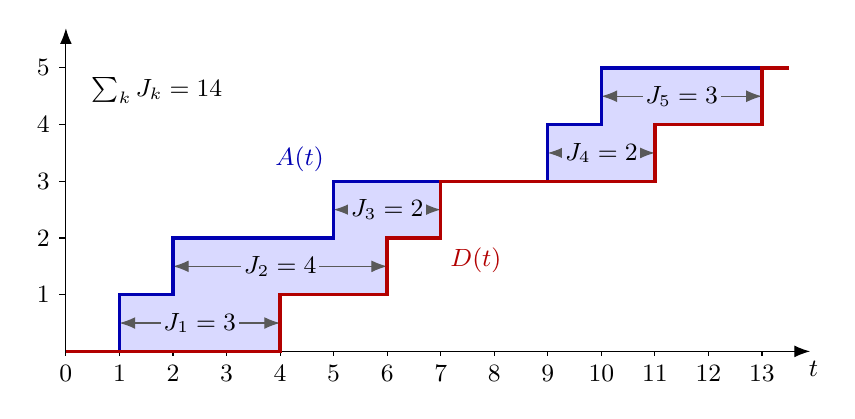
\begin{tikzpicture}[font=\small, >={Latex[length=2mm]}, x=0.68cm, y=0.72cm]
  % strips between the curves
  \foreach \k/\a/\d/\j in {1/1/4/3, 2/2/6/4, 3/5/7/2, 4/9/11/2, 5/10/13/3} {
    \fill[blue!15] (\a,\k-1) rectangle (\d,\k);
    \draw[<->, gray!70!black, thin] (\a,\k-0.5) -- (\d,\k-0.5);
    \node[fill=blue!15, inner sep=1pt] at ({(\a+\d)/2},\k-0.5) {$J_{\k}=\j$};
  }
  % axes
  \draw[->] (0,0) -- (13.9,0) node[anchor=north west, xshift=-4pt] {$t$};
  \draw[->] (0,0) -- (0,5.7);
  \foreach \t in {0,1,...,13} \draw (\t,0) -- (\t,-0.08) node[below] {$\t$};
  \foreach \n in {1,...,5} \draw (0,\n) -- (-0.12,\n) node[left] {$\n$};
  % counting processes
  \draw[blue!70!black, very thick] (0,0) -- (1,0) -- (1,1) -- (2,1) -- (2,2) -- (5,2) -- (5,3)
    -- (9,3) -- (9,4) -- (10,4) -- (10,5) -- (13.5,5);
  \draw[red!70!black, very thick] (0,0) -- (4,0) -- (4,1) -- (6,1) -- (6,2) -- (7,2) -- (7,3)
    -- (11,3) -- (11,4) -- (13,4) -- (13,5) -- (13.5,5);
  \node[blue!70!black, anchor=south east] at (5,3) {$A(t)$};
  \node[red!70!black, anchor=north west] at (7,2) {$D(t)$};
  \node[anchor=west] at (0.3,4.6) {$\sum_k J_k=14$};
\end{tikzpicture}
\end{document}
